\let\negmedspace\undefined
\let\negthickspace\undefined
\documentclass[journal,12pt,twocolumn]{IEEEtran}
\usepackage{cite}
\usepackage{amsmath,amssymb,amsfonts,amsthm}
\usepackage{algorithmic}
\usepackage{graphicx}
\usepackage{textcomp}
\usepackage{xcolor}
\usepackage{txfonts}
\usepackage{listings}
\usepackage{enumitem}
\usepackage{mathtools}
\usepackage{gensymb}
\usepackage{comment}
\usepackage[breaklinks=true]{hyperref}
\usepackage{tkz-euclide} 
\usepackage{listings}
\usepackage{gvv}                                        
\def\inputGnumericTable{}                                 
\usepackage[latin1]{inputenc}                                
\usepackage{color}                                            
\usepackage{array}                                            
\usepackage{longtable}                                       
\usepackage{calc}                                             
\usepackage{multirow}                                         
\usepackage{hhline}                                           
\usepackage{ifthen}                                           
\usepackage{lscape}

\newtheorem{theorem}{Theorem}[section]
\newtheorem{problem}{Problem}
\newtheorem{proposition}{Proposition}[section]
\newtheorem{lemma}{Lemma}[section]
\newtheorem{corollary}[theorem]{Corollary}
\newtheorem{example}{Example}[section]
\newtheorem{definition}[problem]{Definition}
\newcommand{\BEQA}{\begin{eqnarray}}
\newcommand{\EEQA}{\end{eqnarray}}
\newcommand{\define}{\stackrel{\triangle}{=}}
\theoremstyle{remark}
\newtheorem{rem}{Remark}
\begin{document}

\bibliographystyle{IEEEtran}
\vspace{3cm}

\title{11.9.3.3}
\author{EE23BTECH11065 - prem sagar}
\maketitle
\newpage

\bigskip 

\renewcommand{\thefigure}{\theenumi}
\renewcommand{\thetable}{\theenumi}
\textbf{Question}:\\ The 5th,8th and 11th terms of a GP are p,q and s respectively .show that \[q^2=ps\]
\textbf{solution}:
\\first term of a GP= x(0)\\
common ratio of GP=r
\begin{align}
x(n)&= x(0)\,r^{n}, \text{if} n \geq 0
\\x(5)&=x(0)\,r^5
\\x(8)&=x(0)\,r^8
\\x({11})&=x(0)\,r^{11}
\\x(8)\,x(8)=x(0)\,r^8\,x(0)\,r^8
     \\ =x(0)^2\,r^{16}
\\x(5)\,x({11})=x(0)\,r^5\,x(0)\,r^{11}
       \\=x(0)^2\,r^{16}
\\x(8)^2=x(5)\,x({11})
\\q^2=ps
\end{align}
\\\begin{tabular}{|c|c|c|}
\hline
\textbf{symbol}& \textbf{value}& \textbf{description}
\\\hline
\multirow{10}{1em}
\\$x(5)$ &$p$& 5th term of GP 
\\\hline
$x(8)$ &$q$& 8th term of GP
\\\hline
$x({11})$ &$s$& 11th term of GP
\\\hline
\end{tabular}\\
\\\\$u(n)=\begin{cases} 1,& \text{if}\, n\geq 0 \\\ 0,& \text{otherwise} \end{cases}$
\\\\\\\begin{align}x(n)=x(0)\,r^{n}\,u(n)\end{align}
from (10)
\\\\$x(n)=\begin{cases} x(0)\,r^{n} &\text{if}\, n \geq 0\\\ 0,& \text{otherwise}
\end{cases}$
\begin{figure}
    \centering
	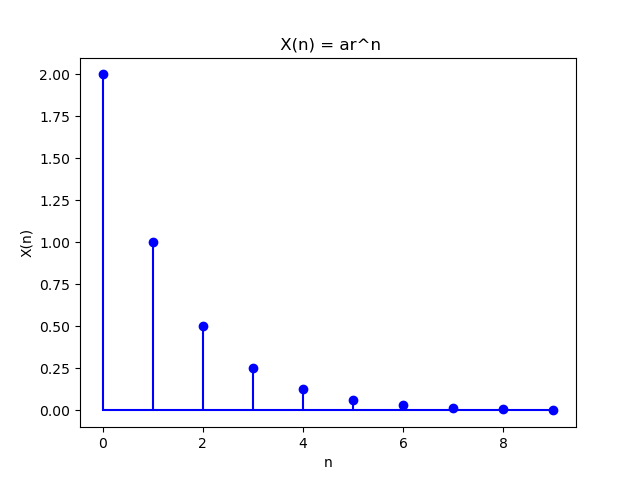
\includegraphics[width=1\linewidth]{geometric_sequence_plot.png}
    \caption{plot x(n) vs n}
    \label{fig:enter-label}
\end{figure}
\\\\\begin{align}x(n)\overset{Z}{\longleftrightarrow}   X(Z)
\\X(Z)&=\sum_{n=-\infty}^{\infty}x(n) Z^{-n}\
     \\ &= \frac{x(0)}{1-r\,z^{-1}}\: \:,|z|>|r| \end{align}   
\end{document}

